\documentclass[a4paper,12pt]{article}
\usepackage[utf8]{inputenc}
\usepackage[ngerman]{babel}
\usepackage[a4paper, left=2.5cm, right=2.5cm]{geometry}
\usepackage{graphicx}
\usepackage{subcaption}
\usepackage{fancyhdr}
\usepackage{pdfpages}
\usepackage{longtable}
\usepackage{multirow}
\usepackage{pgfplots}
\usepackage{pgfplotstable}
\usepackage{float}
\pagestyle{fancy}
\lhead{Messtechnik Labor}
\chead{}
\rhead{Gruppe 2}

\begin{document}
	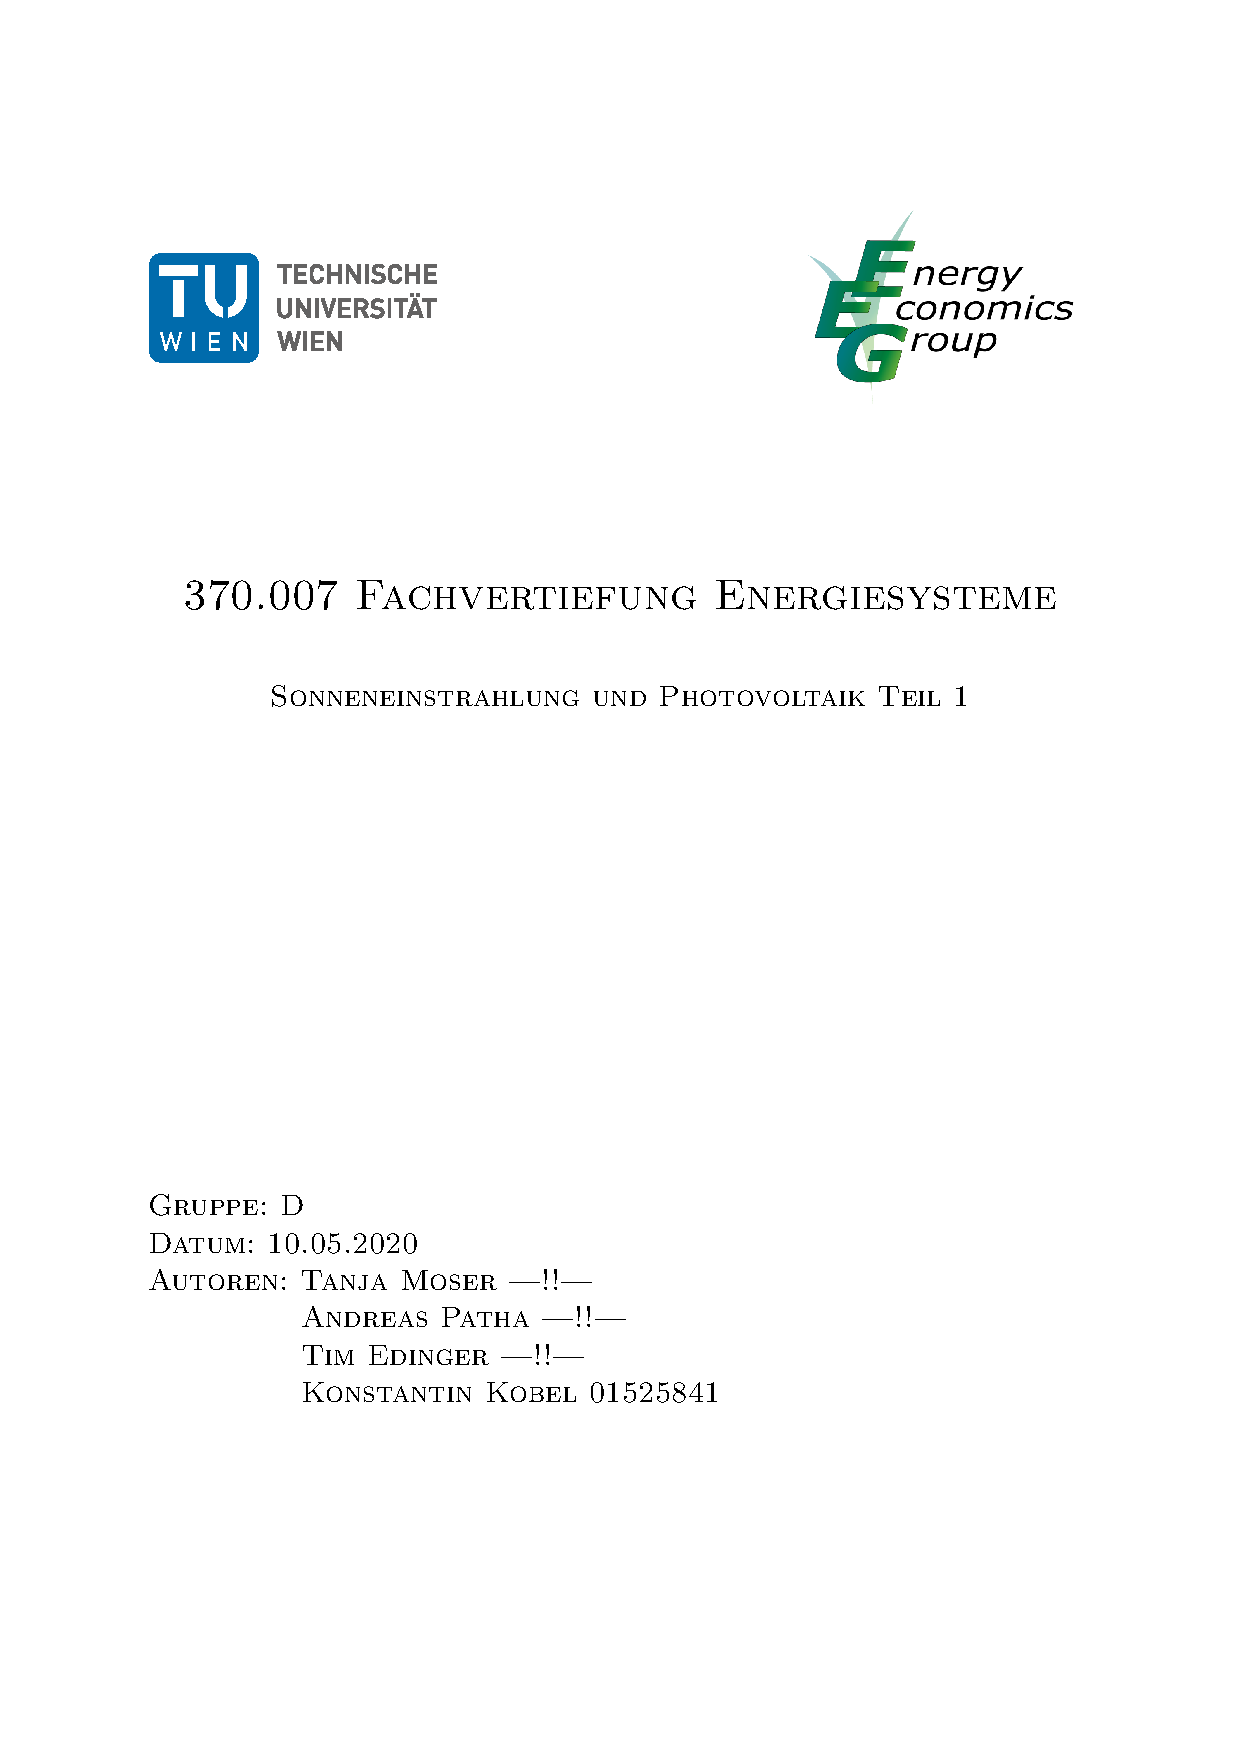
\includepdf{Protokoll_titlepage.pdf}
	
	\newpage
	%Inhaltsverzeichnis
	\tableofcontents
	
	\newpage
	\section{Aufgabenstellung}
	\subsection{Aufgabe 1.1}
	Aufgabe 1.1 befasst sich mit einer PV-Anlage mit folgenden Parametern:
	\begin{itemize}
		\item Der Standort ist Wien ($48.2^{\circ}$N, $16.3^{\circ}$O).
		\item Die installierte Leistung ist $1kWp$.
		\item Der Neigungswinkel der PV-Anlage beträgt $20^{\circ}$.
		\item Der Azimut der Anlage ist $180^{\circ}$ Süden.
		\item Der Modulwirkungsgrad $\eta_{Modul}$ ist $0.17$.
		\item Sonstige Verluste $\eta_{sonst}$ (Reflexion, Temperatur, Wechselrichter, etc.) werden mit dem Wert $0.8$ eingerechnet.
		\item Die Strahlungsdaten für den Standort sind in der Datei $Strahlung.mat$ gegeben.
		\item Die Zeit in Viertelstunden-Werten ist in der Datei $time.mat$ gegeben.
		\item Die Errechnung des Sonnenstandes erfolgt mit der in der Datei $SonnenstandTST.m$ zur Verfügung gestellten Funktion $SonnenstandTST()$.
	\end{itemize}
	Zusätzlich werden folgende Annahmen getroffen:
	\begin{itemize}
		\item Standardtestbedingungen zur Bestimmung des Modulwirkungsgrades bzw. der Nennleistung $P_{peak}$ (in W) bei $25^{\circ}$ Modultemperatur.
		\begin{equation}
			P_{peak}=R_{STC}*A*\eta_{Modul}
		\end{equation}
		\item Vereinfachte Annahme für die Bestimmung des Ertrags der Anlage im Modell.
		\begin{equation}
			E_{ges}=G_{geneigt}*A*\eta_{Modul}*\eta_{sonst}
		\end{equation}
		\item Konstanter Wirkungsgrad.
		\item Erträge bei einem Höhenwinkel unter $5^{\circ}$ werden vernachlässigt.
		\item Konstante Einstrahlung in den 15 Minuten Intervallen.
		\item Norden $5^{\circ}$, Osten $90^{\circ}$, Süden $180^{\circ}$, Westen $270^{\circ}$.
	\end{itemize}
	Die Aufgaben lauten:
	\begin{itemize}
		\item[a)] Erstellen Sie ein Modell, das für den gegebenen Sonnenstand und die Einstrahlungswerte (Diffus- und Direktstrahlung) auf eine horizontale Fläche den Ertrag der PV-Anlage nach Angabe der installierten Leistung in $kW_{peak}$ und der Ausrichtung der Anlage (Azimut und Neigungswinkel) modelliert. Verwenden Sie dazu das isotrope Einstrahlungsmodell.
		\item[b)] Berechnen Sie mit Hilfe der Funktion aus a) den gesamten Jahresertrag 2005 und die Volllaststunden einer $1kWp$ Anlage in Wien.
	\end{itemize}
	\subsection{Aufgabe 1.2}
	Die Unterpunkte der Aufgabe 1.2 lauten:
	\begin{itemize}
		\item[a)] Erstellen Sie die Leistungsdauerlinie der PV-Erzeugung über das Jahr. Sortieren Sie dazu die erzeugte Leistung vom Maximum bis zum Minimum.
		\item[b)] Plotten Sie die monatlichen Erträge der PV-Erzeugung (12 Werte).
		\item[c)] Ermitteln Sie jeweils die 5 Tage mit der minimalen und der maximalen PV-Erzeugung. Geben Sie die Tage (Datum) und den energetischen Ertrag dieser Tage an.
		\item[d)] Stellen Sie in einem Diagramm die Anteile der Diffus-, Direkt- und der reflektierten Strahlung an jedem der 365 Tage dar (verwenden Sie dazu das File $plotStrahlungsanteile.m$).
		\item[e)] Berechnen Sie die durchschnittliche Stromproduktion für jede Stunde am Tag für die Monate Juni und Dezember. Erstellen Sie ein Diagramm mit Boxplots der Erzeugung für jede Stunde des Tages für die jeweiligen Monate.
		\begin{itemize}
			\item Jeder Stundenwert besteht aus der Summe von vier Viertelstundenwerten.
			\item Jeder Monat wird durch eine Matrix mit den Abmessungen $Stunden x Tage$ dargestellt.
			\item Der Input eines Boxplots ist eine Matrix.
		\end{itemize}
	\end{itemize}
	\newpage
	\section{Berechnungen}
	\subsection{Beschreibung der Winkel}
	\begin{figure}[H]
		\centering
		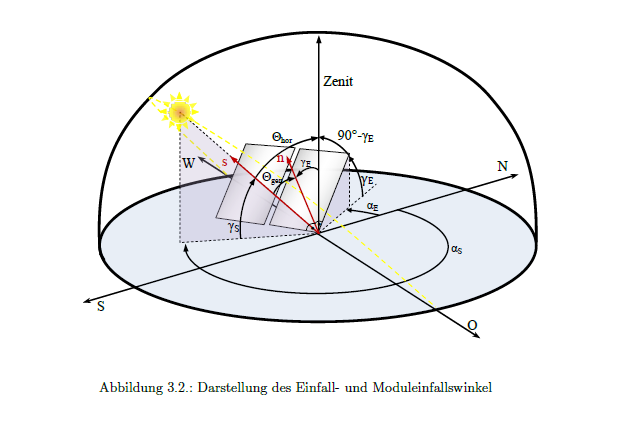
\includegraphics[width=12cm]{img/Winkel}
		\caption{Darstellung des Einfall- und Moduleinfallswinkel.}
	\end{figure}
	\begin{itemize}
		\item $\alpha_S$ - \textbf{Sonnenazimut}. Der Sonnenazimut ist der Winkel zwischen der geographischen Nordrichtung und dem Vertikalkreis durch den Sonnenmittelpunkt. Er ist abhängig von der geographischen Breite des Standorts, der Jahreszeit und der Tageszeit.
		\item $\gamma_S$ - \textbf{Sonnenhöhe}. Die Sonnenhöhe ist der Winkel zwischen dem Sonnenmittelpunkt und der Horizontalebene vom Beobachter. Er ist ebenfalls abhängig von der geographischen Breite des Standorts, der Jahreszeit und der Tageszeit. 
		\item $\alpha_E$ - \textbf{Modulazimut}. Der Modulazimut ist der Winkel der die Modulausrichtung gegenüber dem geographischen Nordpol angibt.
		\item $\gamma_E$ - \textbf{Modulneigungswinkel.}
		\item $\Theta_{gen}$ - \textbf{Moduleinfallswinkel geneigt}. Der Einfallswinkel der Sonnenstrahlung auf eine geneigte Fläche.
		\item $\Theta_{hor}$ - \textbf{Moduleinfallswinkel horizontal}. Der Einfallswinkel der Sonnenstrahlung in horizontaler Richtung.
		\item $Zenit$ - \textbf{Zenit}. Der Zenit steht normal auf den "Horizont".
	\end{itemize}
	\subsection{Berechnung des Moduleinfallswinkels $\Theta_{gen}$}
	Der Moduleinfallswinkel $\Theta_{gen}$ ist für die Berechnung der einzelnen Strahlungsanteile relevant. Er ist von der Südausrichtung des Moduls abhängig.\\
	In unserem Fall beträgt die Südausrichtung $180^{\circ}$. Daraus folgt die Formel zur Berechnung des Moduleinfallswinkels zu
	\begin{equation}
		\Theta_{gen} = \arccos{[-\cos{(\gamma_S)}*\sin{(\gamma_E)}*\cos{(\alpha_S-\alpha_E-180^{\circ})}+\sin{(\gamma_S)}*\cos{(\gamma_E)}]}
	\end{equation}
\end{document}